% !TEX TS-program = pdflatexmk
% !BIB TS-program = bibtex

\documentclass[12pt, a4paper, twoside]{book}
\usepackage{import}
\subimport{../}{preamble}
\ExecuteBibliographyOptions{articletitle=false}
\standalonetrue
\onehalfspacing
\begin{document}

\begin{singlespace}
\color{white}
\chapter{Introduction}
\end{singlespace}

\AddToShipoutPictureBG*{ \AtPageUpperLeft{ \put(0,-240)
{\includegraphics[width=\paperwidth, clip=true, trim=0 250 0 0]{figures/chapter_cover.jpg}}
}}

% Introduction to nanophotonics
Optics has always been one of the primary branches of applied science used to probe and extract information from many physical systems. By studying the way light interacts with a material its properties can be discerned. This is the main principle behind optical microscopy. Conventional optics, solely based upon the use of light, {\color{red}however,} is held back by a fundamental limitation. The finite momentum of the photon restricts the spatial confinement of light to its wavelength. Since the discovery of the diffraction limit in 1873, a great amount of work has been done trying to circumvent the limit it imposes and retrieve information from sub-wavelength emissions. Whilst the diffraction limit is firmly fixed for freely propagating photons it can be broken at an interface, where waves can acquire evanescent character. Such surface waves excitations can exist with wavelengths far below those of photons. By understanding the electromagnetic behaviour of waves on an interface, optics can be brought down to nanoscale dimensions.

Nanophotonics is the name given to the progression of optics into the sub-wavelength domain - the understanding and application of light beyond the diffraction limit. To achieve this nanoscale localisation, nanophotonics exploits light-matter interactions. Matter polarised by an external electromagnetic field can generate its own fields. These fields are determined both by the incident field and by the physical characteristics of the matter. By this mechanism the optical properties of metals on the nm-scale become particularly interesting.

% Plasmons in general
Plasmonics is the study of electromagnetic waves coupled with a metal surface, where collective oscillations of free electrons are considered as excitations of plasmon quasiparticles. By transferring photonic energy into free electron oscillations the limits of optical confinement can be overcome and light can be strongly confined to sub-wavelength dimensions on the surface of the metal in the form of a surface charge density oscillation - a surface plasmon. For this reason plasmonics is sometimes known as \textit{"metal optics"}.
Surface plasmons maintain the same frequency as their photonic excitation, however their wavelength is far below the diffraction limit. This is the first interesting property of the plasmon. Secondly, as light becomes confined to a metallic surface in the form of a plasmon {\color{red}it retains its energy.} Charge accumulates at the surface, thus the electric field surrounding a strongly confined plasmon becomes strongly enhanced. This resonant near-field enhancement is the next most interesting property of a plasmon and the basis for nearly all applications of plasmonics to date.\footnote{The other main exploitation being the resonant position for refractive index sensing.}

% Localised surface plasmons
\begin{figure}[bt]
\centering
\fontsize{10pt}{1em}\selectfont
\def\svgwidth{0.6\textwidth}
\subimport{./figures/}{aunp_plasmon_diagram.pdf_tex}
\def\svgwidth{0.35\textwidth}
\subimport{./figures/}{aunp_optical_antenna.pdf_tex}
\caption[Diagram of a localised surface plasmon in a AuNP.]{\textbf{Diagram of a localised surface plasmon in a AuNP.} Electrons move to screen the external field from the AuNP. The charge density at the electromagnetic poles of the surface greatly enhances the local field. AuNPs are therefore considered to be optical nano-antennae. The electric field from a near-field transmitter is coupled via an antenna into far-field radiation. By reciprocity, far-field radiation can be received in the near-field.}
\label{fig:aunp_plasmon}
\end{figure}

Noble metals have particularly good surface plasmons in the visible region of the electromagnetic spectrum, and are therefore used in the vast majority of all work involving plasmonics. Their electrons are highly mobile and freely move to oppose an incident field, leading to strong collective oscillations of conduction electrons. This is particularly true for collective oscillations confined to the surface of \glspl{mnp}, which develop highly localised fields when resonantly driven by light as a result of surface charge accumulation (\figurename~\ref{fig:aunp_plasmon}). These are known as \glspl{spr} and lead to resonant field enhancement at the plasmon poles. In fact, it is due to the existence of \gls{mnp} \glspl{spr} and noble \gls{mnp} impurities that historically led to the vibrant colouring of stained glass.

As external, far-field light readily couples with plasmons in \glspl{mnp} they have becomes known as optical antennae, in analogy with conventional metal radio wave antennae \cite{novotny2011}. Consequently, they are seen as a simple and efficient method for transferring and confining photonic energy to nanoscale dimensions. Energy can then be transferred to nano-absorbers, such as quantum dots. By reciprocity, near-fields from nano-emitters can be efficiently transferred into the far-field.
% Plasmon interactions
In the event in which the near-fields of two plasmons come into close proximity, energy is transferred between them via an interaction field. As a plasmon is simply a charge oscillation, similar in many cases to a {\color{red}point} dipole, it is susceptible to interactions with other dipoles. This interaction causes the resonant frequency of the coupled system to redshift, and the near-field becomes strongly confined to the space between plasmons. The smaller the space between dielectric and metallic surfaces, the stronger the confinement of light into the dielectric. The result of this compression is a strong increase in the electric field stored within the region. Field strengths can readily increase up to \num{e8} times the incident field \cite{}. Such regions are known as "hot spots" and form the basis for most plasmonic sensing platforms.

% SERS and SNOM - applying the field enhancement
Sensing has become the primary application of plasmonics since its inception. Application of the plasmonic field enhancement has led to the development of now widely used localised optical sensing techniques, good examples of which are \gls{sers} \cite{fleischmann1974, jeanmaire1977} and \gls{snom} \cite{ash1972super, pohl1984optical, lewis1984development, pohl1986optical, harootunian1986super, betzig1988near}. In the same manner that the \gls{spr} spectrally shapes the scattered field, the signature of molecular bonds from optically polarised molecules is imprinted in the scattered field due to inelastic scattering. This is the basic description of Raman scattering \cite{raman1928}. However, since the molecular cross-section is order of magnitudes smaller than the wavelength of light, their coupling, and therefore inelastic scattering is weak. Only 1 in \num{e7} photons are inelastically scattered due to the Raman effect. By coupling photons into plasmons the spatial extent of the near-field becomes comparable to the molecular cross-section and the interaction strength is greatly increased. By reciprocity, electromagnetic fields scattered from molecules in the near-field can be efficiently coupled into far-field photons via mediating plasmons. This is the effect of the field enhancement and the purpose of an optical antenna. By placing molecules in the vicinity of a plasmonic surface and utilising the plasmonic field Raman scattering can be greatly enhanced by $\left|E/E_0\right|^4$.%
\footnote{The amount of scattering depends on the intensity of the illumination $I_{in}=|E_{in}|^2$ and the amount of field scattered back $I_{out} = |E_{out}|^2$, both subject to plasmonic field enhancement ($E_0\rightarrow E_{plasmon} = |E/E_0| E_0$), therefore the total Raman scattering signal is approximated by $I = I_{in}I_{out} \propto I_{in}^2 = |E/E_0|^4$.}
\Gls{snom} is similar in that the near-field is efficiently collected and transmitted into the far-field by a sub-wavelength aperture, a process that can be boosted by plasmonic apertures and, in more recent years, tips. By further increasing the field enhancement in a plasmonic system it has become possible to even detect light scattering from just a few molecules within a single hot spot \cite{zhang2013}.

\begin{figure}[bt]
\centering
\begin{tikzpicture}
\node[anchor=south west] at (-1.3,-1.5) {\includegraphics[width=0.9\textwidth]{data/plasmonic_regimes_background}};
\node[anchor=south west] at (0,0) {\includegraphics{data/plasmonic_regimes_foreground}};
\end{tikzpicture}
\caption[Regimes of plasmonic interaction.]{\textbf{Regimes of plasmonic interaction.} The diagram shows the coupling strength between two plasmonic particles across the full range of characteristic separation dimensions. At distances greater than the particle radius plasmons are uncoupled. Classical mode coupling begins at separations below the particle radius. Many nanoscale phenomena, such as capillary force/surface tension snap-in occur at these characteristic separations. Once the separation transitions to below \SI{1}{nm} quantum mechanical effects begin to become important. The quantum regime is the point at which these effects significantly effect plasmonic interaction.}
\label{fig:plasmonic_regimes}
\vspace{-10pt}
\end{figure}

% Introduction to sub-nm plasmon coupling and the quantum regime
Realistically, this field enhancement can only be boosted so far. By continuing the push the boundaries towards robust single molecule plasmonic sensing, intuition suggests that plasmonic systems must become increasingly smaller to further confine light and further increase the localised near-field enhancement. Inevitably though, the characteristic dimensions of the nano-gaps sustaining the hot spots, or the particles themselves, becomes sufficiently small that quantum mechanical effects, such as quantum tunnelling and non-locality, are no longer negligible and begin to adversely affect confinement (\figurename~\ref{fig:plasmonic_regimes}). Plasmonics in these quantum mechanically-limited regimes currently only has a limited understanding due to difficulty in reliably accessing sub-nm length scales. To a certain extent this is primarily caused by difficulty fabricating structures with such small characteristic features. Few reports have therefore conclusively shown the influence of quantum effects on plasmonic performance and it remains an interesting and relatively new region of plasmonics that still requires exploring.

% The correct measurements to understand the quantum regime
The ideal way of experimentally mapping the quantum regime is to use precisely positioned individual nanoparticles coming closer together, in a similar manner as theoretical studies, and transitioning from classical to quantum to contacted interaction regimes. Though possible in many ways, the dynamic control and precise positioning of a sub-nm cavity between two nanoparticles is not a trivial task. While there are methods for controlling nanoparticle positions, difficulty arises as to what measurements are then possible. A rich amount of fundamental physics exists within sub-nm gaps that can strongly influence plasmonic behaviour, therefore a system must be carefully designed to enable measurement of each significant effect. Sensitive measurements of charge transfer and forces, not compatible with individual nanoparticle experiments, are required to probe both plasmonic and quantum mechanical effects. Consequently, precise nanopositioning of an electrically contacted nanoparticle with force sensitivity is required in order to experimentally access and improve the understanding of a regime in which quantum effects influence plasmonics.

% The use of tips for plasmonics
AFM probes are appealing devices as a means of controllably progressing into the sub-nm regime whilst simultaneously making the necessary measurements to understand the quantum regime, though a plasmonic tip apex structure is a necessity. Metallic tip structures at a glance are promising plasmonic probes as  characteristic apex dimensions readily fall well below the diffraction limit. Furthermore, a clear advantage of tip systems is the maturity of the many surface science techniques used for characterising nanoscale topology, forces and electronic properties. Techniques such as \gls{stm} \cite{binnig1982} and \gls{afm} \cite{binnig1986} have formed the foundation of surface analysis studies since their inception. By combining the measurements possible using \gls{afm} probes with optical studies further insight into the quantum regime can be gained. This was the approach adopted by Savage \text{et al.} to initially investigate the effect on the plasmonics caused by the onset on electron tunnelling \cite{savage2012}.

\section{Project Outline}

The primary purpose of this project is to demonstrate robust measurements of plasmonic gaps in the sub-nm regime, at the point when quantum effects become important, building upon the work done by Savage \textit{et al.} \cite{savage2012}. A modified microscope design is employed compared to that used by Savage \textit{et al.} to incorporate a larger range of possible measurements and potential experiments. By using a combined atomic force-optical microscope and two opposing, plasmonic tips, plasmons can be dynamically probed using multiple, simultaneous, correlated measurements. A large amount of time and effort has been dedicated to the design and {\color{red}development/construction} of a microscope capable of making simultaneous measurements of the electronic, force and optical signals from a plasmon tip dimer in order to better understand the quantum regime of tunnelling plasmonics. Both the microscope technology and the sample fabrication technology are heavily developed to enable robust measurements on sub-nm gaps and improve upon the current standards of experiment.

A prerequisite of all experiments is the availability of plasmonic AFM tips with far-field surface plasmon resonances, the simplest geometry of which is a spherical tip apex. Spherical AuNPs mounted onto two conductive AFM tips are used to dynamically form plasmonic nano-gaps. Though studies are carried out on commercially available spherical Au tips the sensitivity of measurements in the sub-nm regime requires more resistant probes. Despite the widespread use of tips in metal optics techniques, the application of nanostructured (optical antennae) probes for improved performance is a relatively new idea. Little work has been reported on the modification of the sharp tip geometry and spherical apex modification remains complex and expensive. To address these issues, a new fabrication technique using electrodeposition is developed as a simple method for producing spherically nanostructured metallic tips.

Prior to their use in fundamental quantum plasmonics experiments, both commercially-available vacuum-processed spherical Au tips and electrochemically-deposited AuNP tips are optically characterised to understand the relation between their plasmons and their ability to act as optical antennae. Their improved field enhancing property over the conventional sharp metallic tip geometry is also demonstrated to further show that such tips can be used outside of fundamental physics experiments.

Finally, with all experimental components in place, the plasmonic response of sub-nm gaps is investigated. Current experiments in the quantum regime of tunnelling plasmonics build upon both previous experimental efforts and the proposed theoretical foundations emerging in recent years to show that atomic-level gap morphology is a dominant factor effecting the fundamental degree to which light can be confined.

% The outline of the chapters
This report necessarily begins with the theoretical background required to understand plasmons and the relevant plasmonic phenomena discussed throughout this text/ within the scope of this project. The previous uses of tips for plasmonics, along with their current understanding, are detailed to motivate their use in experimental plasmonics.
The experimental work carried out in this project is discussed in three parts: the production of plasmonic spherical-apex AFM tips by electrochemical nanostructuring, the design and construction of a microscope capable of making stable measurements on an AFM tip dimer in the sub-nm regime, and finally the results of the experiments using the combination of the two. These results are broken down into understanding the plasmonics of individual nanostructured tips followed by understanding of the coupling between two tips as their separation progresses into the sub-nm quantum regime.

\ifstandalone
\begin{singlespace}
\fontsize{8pt}{1em}\selectfont
\printbibliography[notcategory=fullcited]
\end{singlespace}
\fi

\end{document}